%----------------------------------------------------%
%           Written by Gaurav Gupta                  %
%    SC21B026, Aerospace Engineering (2021 Batch)    %
%       Inspired by the CALTECH Beamer Theme         %
%----------------------------------------------------%

\documentclass[hyperref={bookmarks=false},aspectratio=169, 10pt]{beamer}
\usepackage[utf8]{inputenc}

%-------------------------Packages------------------------
\usepackage[spanish]{babel}
\usepackage[utf8]{inputenc}
\usepackage{subcaption}
\usepackage{amsmath}
%---------------------------------------------------------
% -----------Define theme and color scheme----------------

\usetheme[sidebarleft]{IIST}  % 3 options: minimal, sidebarleft, sidebarright

% ---------Information on the title page------------------
\title[Muestreo estratificado]
{\bfseries{Muestreo estratificado}}

\author[]{Aurora Rios Medina

Jose Manuel Gonzalez Alcantara

Juan Carlos Escobar Teja

Osmar Dominique Santana Reyes}

\date[Oct, 2024]{\today}
%------------------------------------------------------------

%------------------------------------------------------------
%The next block of commands puts the table of contents at the beginning of each section and highlights the current section:

% \AtBeginSection[]
% {
%   \begin{frame}
%     \frametitle{Table of Contents}
%     \tableofcontents[currentsection]
%   \end{frame}
% }
%------------------------------------------------------------

\begin{document}

\frame{\titlepage}  % Creates title page

%--------table of contents after title page---------------

%---------------------------------------------------------

\section{4.1. ¿Qué es el muestreo estratificado?}

%---------------------------------------------------------
%Changing visivility of the text
\begin{frame}
\frametitle{4.1. ¿Qué es el muestreo estratificado?}
    Muchas veces se cuenta con información extra acerca de una población, que puede ayudar a obtener una muestra más representativa. Por ejemplo,

    \begin{minipage}[t]{0.4\linewidth}
        \begin{itemize}
            \item Al realizar una muestra sobre una población dada, para saber sobre el consumo de alimentos en la población. 
            
            %
\includegraphics[width = 0.9\linewidth]{MujervsHombre.jpg}
        \end{itemize}
    \end{minipage} \hspace{0.05\linewidth}
    \begin{minipage}[t]{0.45\linewidth}
        \begin{itemize}
            \item Los residentes rurales acuden más a una tienda que los residentes urbanos.
            
            %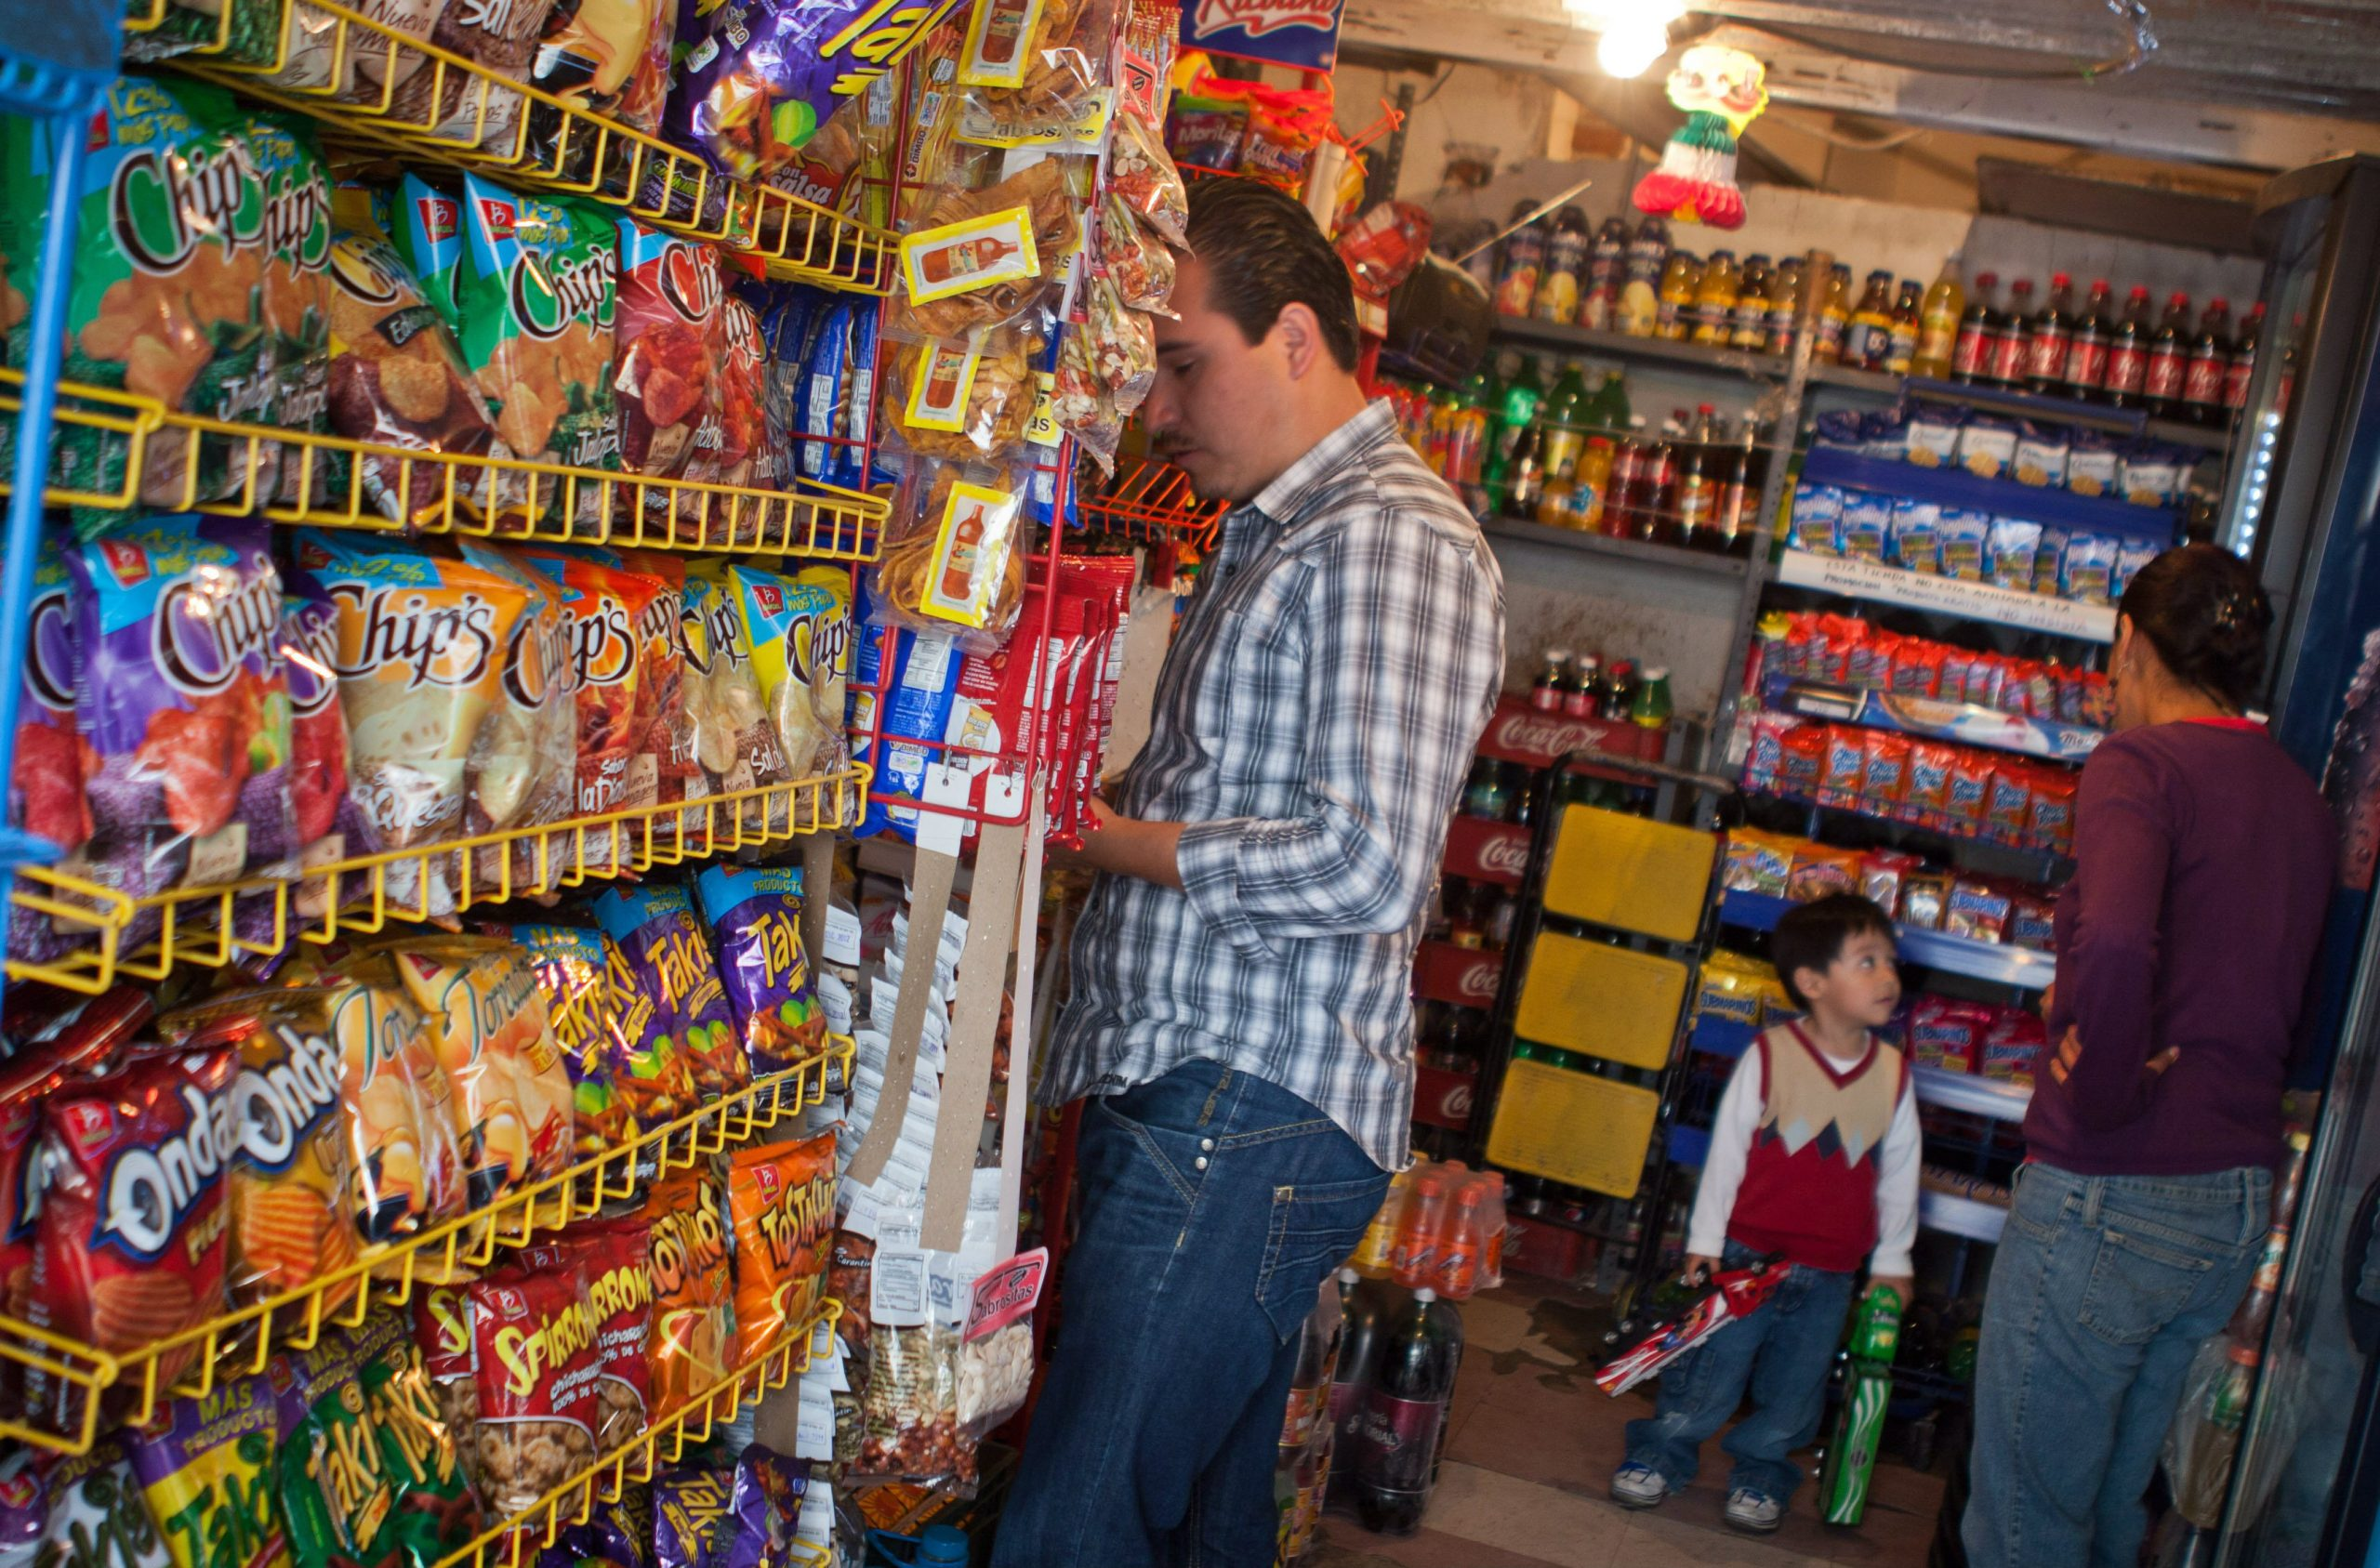
\includegraphics[width = 0.9\linewidth]{tienda.jpg}
        \end{itemize}
    \end{minipage}
\end{frame}

%---------------------------------------------------------

%---------------------------------------------------------
%Highlighting text
\begin{frame}
    \frametitle{4.1. ¿Qué es el muestreo estratificado?}
  
    Sea $ \Omega $ una población finita de $ N $ elementos y $ \left\lbrace \Omega_1, \Omega_2, \ldots, \Omega_m \right\rbrace $ una partición de $ \Omega $. A cada $ \Omega_i $, con $ i = 1, \ldots, m $ se le llama \textbf{estrato de la población}. 

    Para cada $ i = 1, \ldots, m $, sean $ N_i = \left| \Omega_i \right| $ y $ n_i $ el tamaño de una muestra obtenida de $ \Omega_i $. Las muestras obtenidas de cada estrato se juntan para formar una muestra de la población total, $ \Omega $. \vspace{3mm}
    
    \textbf{Observaciones:}

    \begin{itemize}
        \item<1-> $ \displaystyle \sum_{i=1}^{m} N_i = N $
        \item<2-> Los métodos de muestreo utilizados en cada estrato no tienen que ser iguales y pueden ser independientes o no.
        \item<3-> Cuando las muestras de cada estrato sean aleatorias, al procedimiento completo se le llamará \textbf{Muestreo aleatorio estratificado}.
    \end{itemize}
\end{frame}

%---------------------------------------------------------

\begin{frame}
    \frametitle{Razones para usar el muestreo estratificado}

    \begin{itemize}
        \item<1-> Obtener mejores muestras en una población. Por ejemplo, si se extrae una muestra aleatoria de tamaño 100 de una población de 2000 estudiantes, donde la mitad son mujeres y la otro mitad hombres, entonces la muestra podría no representar bien a la subpoblación de mujeres o a la de hombres. Por lo tanto, sería mejor optar por extrar una muestra de 50 hombres y otra de 50 mujeres.
        \item<2-> Se desean obtener datos de precisión conocida sobre las subpoblaciones. Por ejemplo, si hay interés en conocer las experiencias educativas y laborales de egresados de cierta carrera, pero también se desea comparar las experiencias de hombres con las de mujeres, un muestreo estratificado sería de utilidad, pues permite estudiar a los egresados en su conjunto y también de forma separada.
    \end{itemize}
\end{frame}

%---------------------------------------------------------

\begin{frame}
  \frametitle{Razones para usar el muestreo estratificado}
    \begin{itemize}
        \item<1-> Para minimizar los costos de obtener información. Por ejemplo, si desea obtener datos sobre las escuelas preparatorias del Estado de México, pero se desean minimizar costos (transporte, comida, artículos de papelería, salarios, etc.), entonces se pueden dividir al conjunto de escuelas de acuerdo a su ubicación. Así, entre más lejos estén, más costo tendrá recabar datos de estas, e inversamente, cuanto más cerca estén, menos gasto se tendría. 
        \item<2-> Si el muestreo estratificado se hace correctamente, entonces las estimaciones sobre la población serán más precisas. Por ejemplo, si se desea estudiar la presión sanguínea de cierta población, sería útil estratificarlas de acuerdo a sus edades, puesto que la presión sanguínea de las personas varía de acuerdo a la edad.
    \end{itemize}
\end{frame}

%---------------------------------------------------------

\begin{frame}
  \frametitle{Ejemplo 4.1}
    Se desea estimar la cantidad promedio de acres agrícolas por condado en Estados Unidos. Para esto se estratificará el país en las zonas noreste, norte-centro, sur y oeste. Se extraerá una muestra aleatoria cercana al 10$\%$ de cada región. Los datos sobre este muestreo se muestran a continuación:

    \begin{table}
        \centering
        \begin{tabular}{|c|c|c|}
            \hline
            \textbf{Estrato} & \textbf{Condados en el estrato} & \textbf{Condados en la muestra}\\
            \hline
            Noreste & 220 & 21 \\
            \hline
            Norte-centro & 1054 & 103 \\
            \hline
            Sur & 1382 & 135 \\
            \hline
            Oeste & 422 & 41 \\
            \hline\hline
            Total & 3078 & 300 \\
            \hline
        \end{tabular}
    \end{table}
\end{frame}

%---------------------------------------------------------

\begin{frame}
    \frametitle{Ejemplo 4.1}
      Una ves extraídas las muestras, se obtinen los siguientes datos:
  
      \begin{table}
          \centering
          \begin{tabular}{|c|c|c|c|}
              \hline
              \textbf{Región} & \textbf{Tamaño de la muestra} & \textbf{Promedio} & \textbf{Varianza}\\
              \hline
              Noreste & 21 & 97,629.8 & 7,647,472,708 \\
              \hline
              NOrte-centro & 103 & 300,504.2 & 29,618,183,543 \\
              \hline
              Sur & 135 & 211.315 & 53,587,487,856 \\
              \hline
              Oeste & 41 & 662,295.5 & 396,185,950,266 \\
              \hline
          \end{tabular}
      \end{table}
\end{frame}

\begin{frame}
  \frametitle{Ejemplo 4.1}
    Como las muestras fueron aleatorias, el promedio de acres agrícolas para cada estrato y su varianza se puenen estimar mediante: $ \hat{t} = N  \overline{y} $ y $\displaystyle V[\hat{t}] = N^2 \left( 1 - \dfrac{n}{N} \right) \dfrac{s^2}{n} $. La siguiente tabla muestra los promedios y varianzas por región:

    \begin{table}
        \centering
        \begin{tabular}{|c|c|c|}
            \hline
            \textbf{Estrato} & \textbf{Total estimado de acres agrícolas} & \textbf{Varianza estimada del total}\\
            \hline
            Noreste & 21,478,558 & 1.59432 $\cdot \, 10^{13}$ \\
            \hline
            Norte-centro & 316,731,379 & 2.88232 $\cdot \, 10^{14}$ \\
            \hline
            Sur & 292,037,391 & 6.84076 $\cdot \, 10^{14}$ \\
            \hline
            Oeste & 279,488,706 & 1.55365 $\cdot \, 10^{15}$ \\
            \hline\hline
            Total & 90,736,034 & 2.5419 $\cdot \, 10^{15}$ \\
            \hline
        \end{tabular}
    \end{table}

    De esta manera, la cantidad total estimada de acres destinados a la agricultura es: 909,736,034 con un desviación estándar de 50,417,248. Así, la cantidad de acres destinados a la agricultura por condado es 909,736,034/3078 = 295,560.7649, con un desviación estándar de 50,417,248/3078 = 16,379.87.
\end{frame}

%---------------------------------------------------------

\begin{frame}
    \frametitle{Ejemplo 4.1}

    Los resultados de realizar un muestreo aleatorio simple en el ejemplo anterior son: una estimación de 916,927,110 acres destinados a la agricultura con una desviación estándar de 58,169,381.

    Así, la ganancia relativa del muestreo por estratificación respecto al muestreo aleatorio simple es:

    \begin{equation*}
        \dfrac{\mbox{varianza estimada de la estratificación}}{\mbox{varianza estimada de la muestra aleatoria simple}} = \dfrac{2.5419 \cdot \, 10^{15}}{3.3837 \cdot \, 10^{15}} \approx 0.75
    \end{equation*}

    Es decir, si estas cifras fueran las varianzas de la población, sería de esperarse que solo se ncesitarán (300)(0.75) = 225 observaciones con muestra estratificada para obtener la misma precisión que con una muestra aleatoria simple de 300 observaciones.
\end{frame}

\frame{}

\end{document}